% Chapter X

\chapter{Simulating Collisions in Thermal Gases} % Chapter title

\label{ch:inhomogas} % For referencing the chapter elsewhere, use \autoref{ch:inhomogas} 

%----------------------------------------------------------------------------------------

Need to introduce the usefulness of the method here. References to many kinds of applications and such things. I also need to perform a literature review of all DSMC used in cold atoms physics.

Compare to molecular dynamic approaches, when is DSMC appropriate / good? When does it fail? 

Find out the knudsen number for typical cold atom conditions. Wade has numbers for stamper kern and shvatchuck.

DSMC - Birds Book \cite{Bird1994}

Evaporative Cooling and Expansion Dynamics: \cite{Wu1996, Wu1997, Wu1998}

Bosonic Collective-Mode dynamics: \cite{Jackson2001, Jackson2001b, Jackson2002, Jackson2002b, Jackson2002c}, Can't find Jackson Zaremba 2002 Laser Physics, 12, 93

Fermion Dynamics: \cite{Urban2006, Urban2007, Urban2008, Lepers2010} (see also \cite{Vignolo2002, Toschi2003, Capuzzi2004, Toschi2004})

Sympathetic Cooling: \cite{Barletta2010, Barletta2011}

Applications - Rayleigh Bernard Flow: \cite{Watanabe1994}

Spacecraft aerodynamics: \cite{Oran1998}

Chemical reactions: \cite{Anderson2003} Goldsworthy?

Microfluidics: \cite{Frangi2003}

Acoustics on Earth, Mars and Titan: \cite{Hanford2009}

Volcanic plumes on Jupiter: \cite{Zhang2004}

Read: \sout{\cite{Minguzzi2004}}, [45]

Refer to cuda section \ref{ch:cudadsmc} Should also discuss the development of this parallel implementation of the code. Compare to CPU implementations. Goldsworthy has a few references for other CUDA codes.

The heart of the DSMC method is to simplify the simulation of interparticle interactions in the form of two body collisions.
In this sense there are two aspects we need to ensure are modelled accurately; the number and frequency of collisions (collision rate) and the collisions themselves, wether or not they are correctly distributing the kinetic energy.
In the following sections I carefully analyse these two aspects to ensure the utmost accuracy in our simulations.

%----------------------------------------------------------------------------------------

\section{Collision Rates in Thermal Gases}

Overall collision rate, spatial collision rate, talk about number of cells, the occupancy of cells and the effect of inhomogeniety.
 
One of the most basic tests for the application of the DSMC method to cold atom physics is to investigate the collision rate for a thermal gas. 
Using the Boltzmann equation we can derive \cite{Walraven2010} the thermally averaged collision rate per unit density for a single species atomic gas bound by the potential ${\cal U}(\mathbf{r})$,
\marginpar{Maybe say something about the Boltzmann equation here and give some references.}
\begin{equation}
    {\tau_c}^{-1} = \frac{1}{2} n_{0}\langle v\sigma \rangle \frac{V_{2e}}{V_e},
\end{equation}
where $n_0 = N / V_e$ is the central density of the gas, $\langle v\sigma \rangle$ is the thermally averaged product of the atomic velocity and collision cross section, $V_e = \int \exp\left[-{\cal U}(\mathbf{r})/kBT\right]\, d\mathbf{r}$ is the effective volume of the gas, and $V_{2e} = \int \exp\left[-2{\cal U}(\mathbf{r})/kBT\right]\, d\mathbf{r}$ the effective volume corresponding to the distribution of pairs.
\marginpar{ The effective volume, $V_e$, of an inhomogeneous gas equals the volume of a homogeneous gas with the same number of atoms and density. }
For the bulk of this work we will consider collisions in three unique trapping potentials: no trapping potential, \ie a homogeneous gas, an Ioffe Pritchard trap(cite) and a spherical quadrupole trap(cite - is it really spherical?)\footnote{We have a more in depth discussion of magnetic trapping in appendix \ref{sec:magneticTrapping}.}.
The simplest scenario we can use to investigate the effects of changing the free parameters is that of a homogeneous gas. 
In this case the collision rate simply reduces to 
\begin{equation*}
    {\tau_{c,\mathrm{box}}}^{-1} = \frac{1}{\sqrt{2}}n_0\bar{v}\sigma,
\end{equation*}
where $\bar{v}=\sqrt{8k_{B}T/\pi m}$, is the average speed of the atoms\footnote{It is interesting to note that the average velocity of the atoms depends only on the temperature of the gas. It is completely \emph{independent} of position and trapping potential. In appendix \ref{sec:thermalPhysics} we have carefully derived this expression for the average velocity of atoms.}. In this case the effective volume, $V_e$, is simply the volume of the box, $V$.

If we use the expression, \eqref{eq:ipmag}, for the magnetic field produced by an Ioffe Pritchard trap from section \ref{sec:intromag} we find the collision rate to be
\begin{equation*}
    {\tau_{c,\mathrm{IP}}}^{-1} = \frac{1}{4}n_0\bar{v}\sigma.
\end{equation*}
However this time the expression for the effective volume is a little more complex
\begin{equation*}
    V_{e,\mathrm{IP}} = \frac{1}{\sqrt{B''}B_\rho''}\left(\frac{4 \pi k_B T}{g_s \mu_B}\right)^{3/2}.
\end{equation*}
We can combine these two equations to form an expression explicit in the temperature and trapping parameters
\begin{equation}
    {\tau_{c,\mathrm{IP}}}^{-1} = \sqrt{B''}B_\rho'' \frac{N \left(g_s \mu_B\right)^{3/2}\sigma}{8\pi^2\sqrt{2m}k_BT}.
\end{equation}
The interesting thing to note here is that the collision rate \emph{increases} as the temperature \emph{decreases}, which is the converse to the homogeneous gas. This is because for a trapped gas the density 

\begin{table}
\myfloatalign
\begin{tabularx}{\textwidth}{|l|c|c|c|} \toprule
\tableheadline{Trapping Potential} & \tableheadline{Trap Power} & \tableheadline{Effective Volume, $V_e$} & \tableheadline{ Collision Rate, ${\tau_c}^{-1}$} \\ \midrule
Homogeneous Gas & 0 &  V & $\frac{1}{\sqrt{2}}n_0\bar{v}\sigma$ \\
\midrule
Spherical Quadrupole & 1 & $256\left(\frac{\pi k_B T}{g_s \mu_B B_z}\right)^3$ & $\frac{1}{8\sqrt{2}}n_0\bar{v}\sigma$ \\
\midrule
Ioffe Pritchard & 2 & $\frac{1}{\sqrt{B''}B_\rho''}\left(\frac{4 \pi k_B T}{g_s \mu_B}\right)^{3/2}$ & $\frac{1}{4}n_0\bar{v}\sigma$ \\
\midrule
Power Law & $3/\gamma$ & $\frac{4}{3}\pi{r_e}^3\Gamma\left[\gamma+1\right]\left(\frac{k_B T}{{\cal U}_0}\right)^{\gamma}$ & $\frac{1}{2^{\gamma+0.5}}n_0\bar{v}\sigma$\\
\bottomrule
\end{tabularx}
\caption[Autem timeam deleniti usu id]{Collision rates for different trapping potentials.}  
\label{tab:example}
\end{table}

%----------------------------------------------------------------------------------------

\section{DSMC simulations of collisions}

The DSMC method offers some free parameters which we can optimise to balance the accuracy and efficiency, namely the number of cells, $n_c$, and the number of test particles, $N_p$.
We wish to see the effect of varying these parameters on the results of the simulation.

**Include a surface plot of the collision rate as a function of cell number and test particle number.
Should make the z axis percentage error. See fig 14. in wade. **

\begin{figure*}
\hspace{-12.5em}
\makebox[1.8\linewidth][l]{%
\centering
\subfigure{\label{fig:a}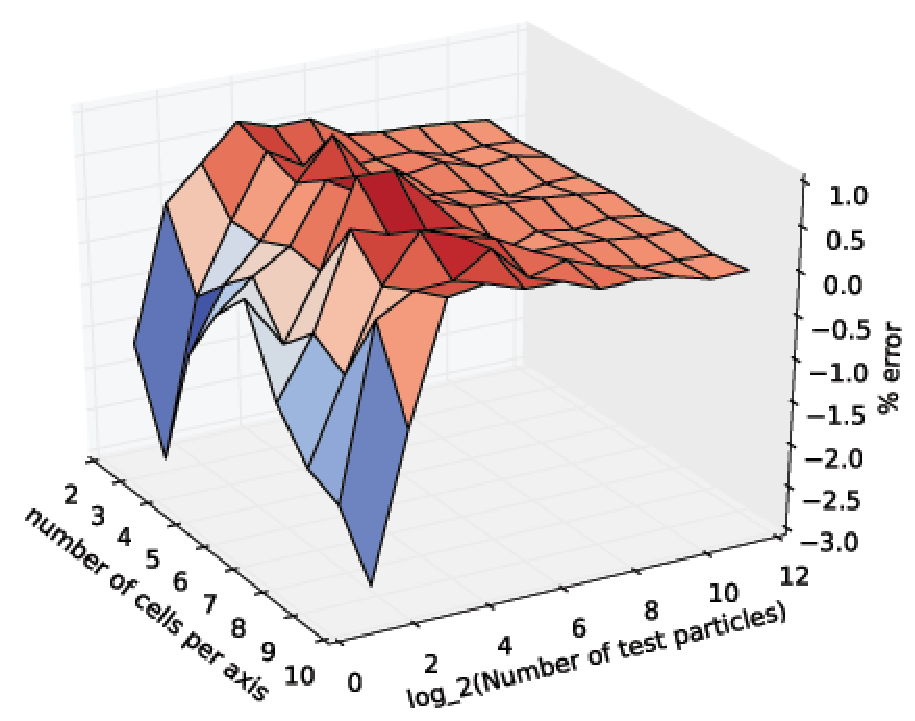
\includegraphics[width=0.525\textwidth]{gfx/HomoError}}%
\subfigure{\label{fig:b}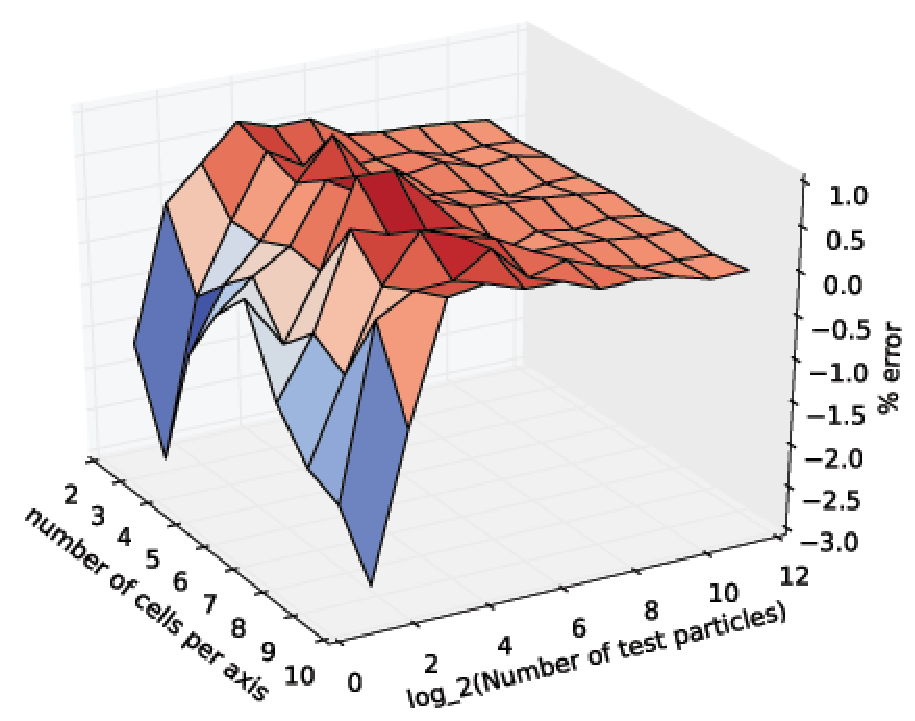
\includegraphics[width=0.525\textwidth]{gfx/HomoError}}%
\subfigure{\label{fig:c}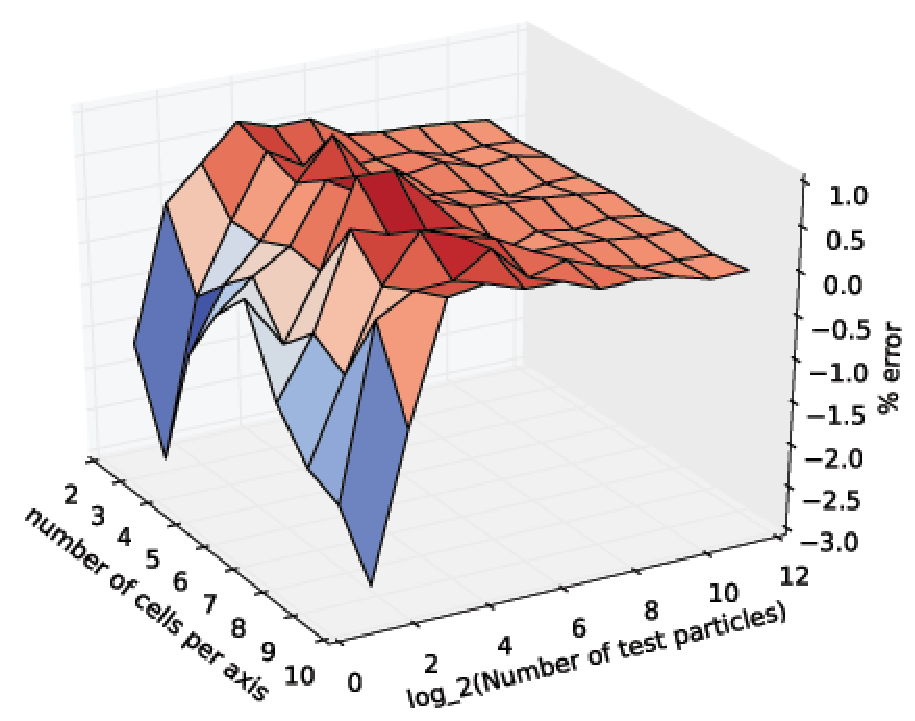
\includegraphics[width=0.525\textwidth]{gfx/HomoError}}%
}
\caption{Error of DSMC method as a function of test particle number and cell number.}\label{fig:dsmccolerr}
\end{figure*}

Figure \ref{fig:dsmchomoerr} shows how well the DSMC method performs over a wide range of test particle and cell numbers. 
We can see in the corner the method beginning to fail. 
This is the region where, on average, we have less than two test particles per cell. 
This means that there is not enough atoms to perform a collision within a cell. 
One way to avoid this (which has not been implemented here) is to search neighbouring cells for collision pairs when a partner can not be found in the current cell.
The main thing to observe here is the increase in the error as the number of test particles is reduced.


%----------------------------------------------------------------------------------------

\section{Thermalisation}

\cite{Davis1995}, \cite{Anderlini2006}

\subsection{Walraven Thermlisation}
In \cite{Walraven2010} we are shown that if we perturb the energy of a small fraction of atoms in a single component gas then the rethermalisation time is given by
\begin{equation}
    \tau_{th}^{-1} = \frac{1}{2\left(\gamma + 3/2\right)} \tau_{c}^{-1},
\end{equation}
where $\gamma$ describes the geometry of the trap. For a homogeneous, harmonic and linear trap $\gamma$ is equal to 0, 3/2 and 3 respectively. Thus we would expect these traps to thermalise in 3, 6 and 9 collision times.

\begin{figure}[bth]
\myfloatalign
\subfloat[Walraven homegeneous gas thermalisation. $\tau_{c}^{-1} / \tau^{-1} = 1.2$ should equal 3? ]
{\label{fig:dsmchomoerr}
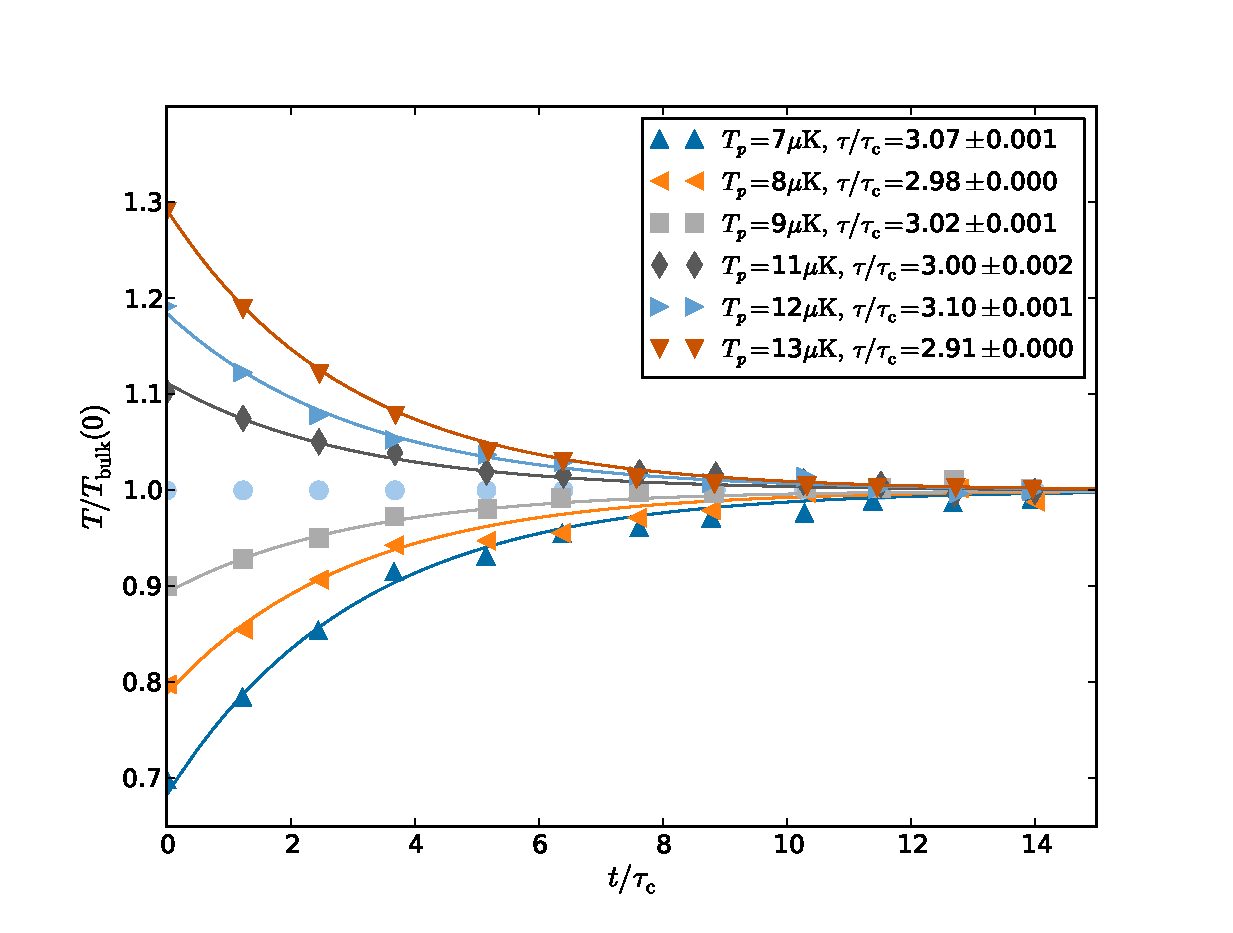
\includegraphics[width=.45\linewidth]{gfx/Thermalisation/walravenHomo}} \quad
\subfloat[Walraven ip gas thermalisation. $\tau_{c}^{-1} / \tau^{-1} = 1.6$ should equal 6?]
{\label{fig:dsmcquaderr}
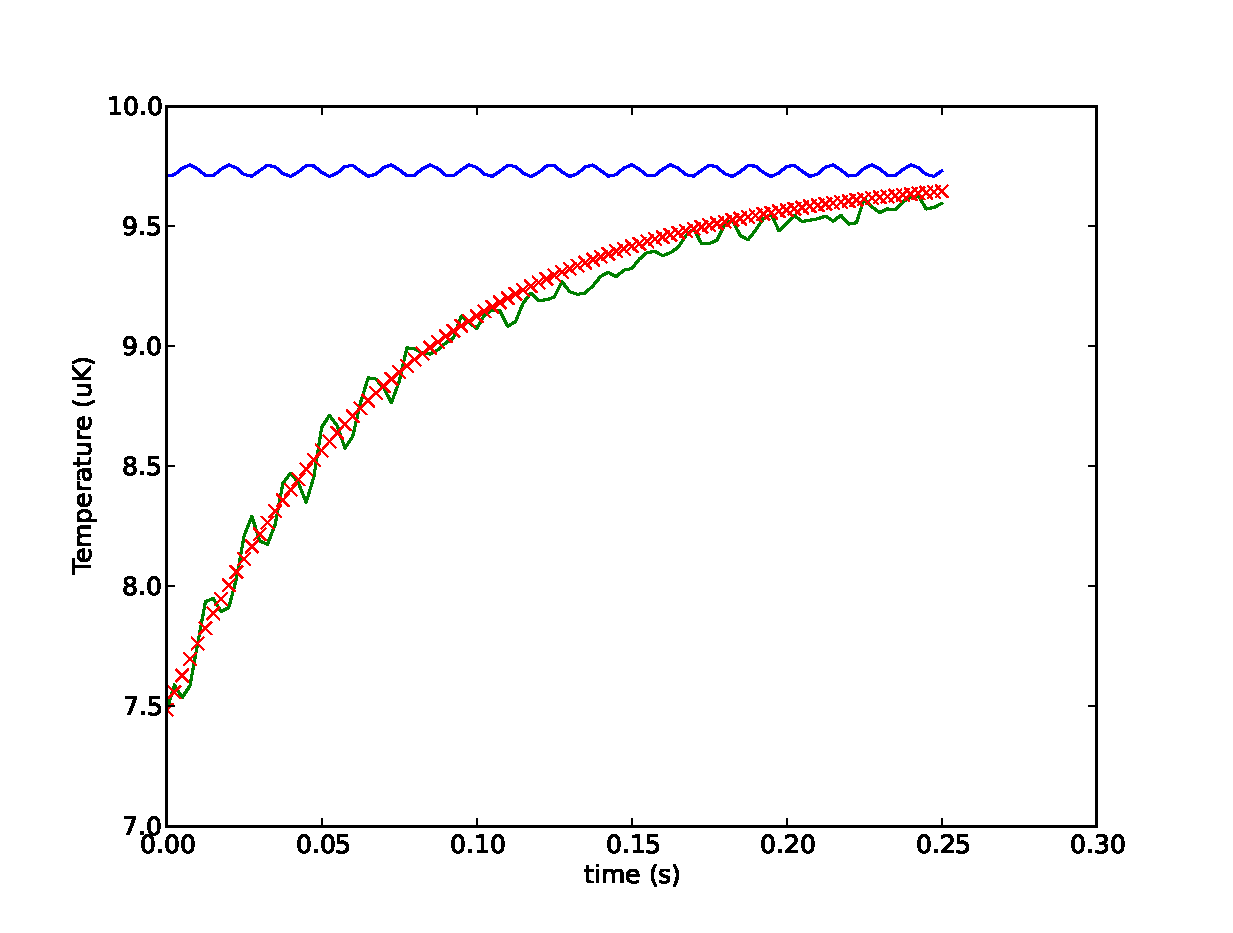
\includegraphics[width=.45\linewidth]{gfx/Thermalisation/walravenIP}}
\subfloat[Walraven quad gas thermalisation. $\tau_{c}^{-1} / \tau^{-1} = 10.45$ should equal 9?]
{\label{fig:dsmcquaderr}
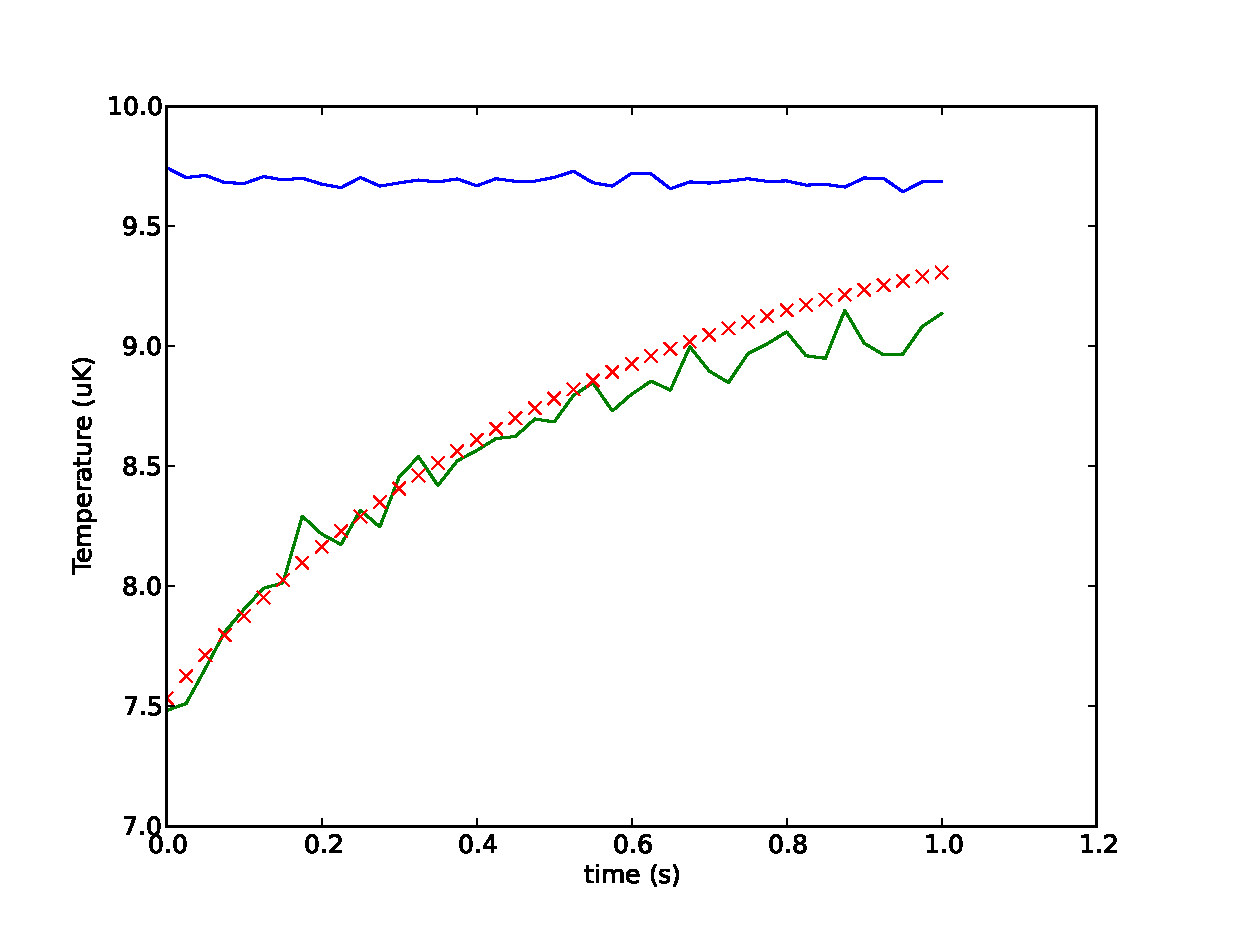
\includegraphics[width=.45\linewidth]{gfx/Thermalisation/walravenQuad}}
\caption[]{Error of DSMC method as a function of test particle number and cell number.}\label{fig:dsmccolerr}
\end{figure}

\subsection{Monroe Thermalisation}
Also simulations of Monroe et al.
I need to somehow think about this problem analytically.
Is there anyway to find an analytic expression for this directional thermalisation?

\begin{figure}[bth]
\myfloatalign
\subfloat[Monroe homegeneous gas thermalisation. $\tau_{c}^{-1} / \tau^{-1} = 0.77$ ]
{\label{fig:dsmchomoerr}
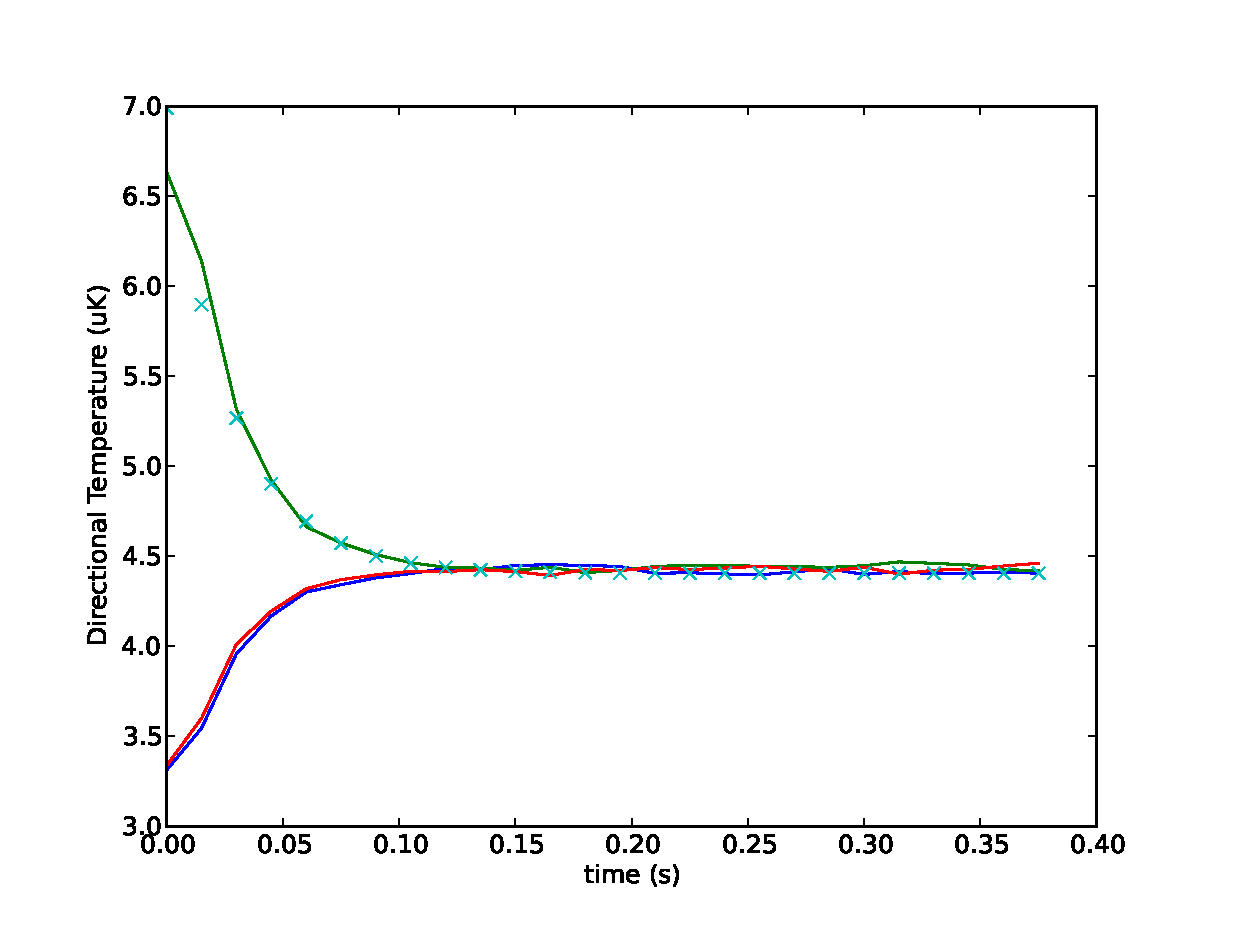
\includegraphics[width=.45\linewidth]{gfx/Thermalisation/monroeHomo}} \quad
\subfloat[Walraven homegeneous gas thermalisation. $\tau_{c}^{-1} / \tau^{-1} = 2.21$]
{\label{fig:dsmcquaderr}
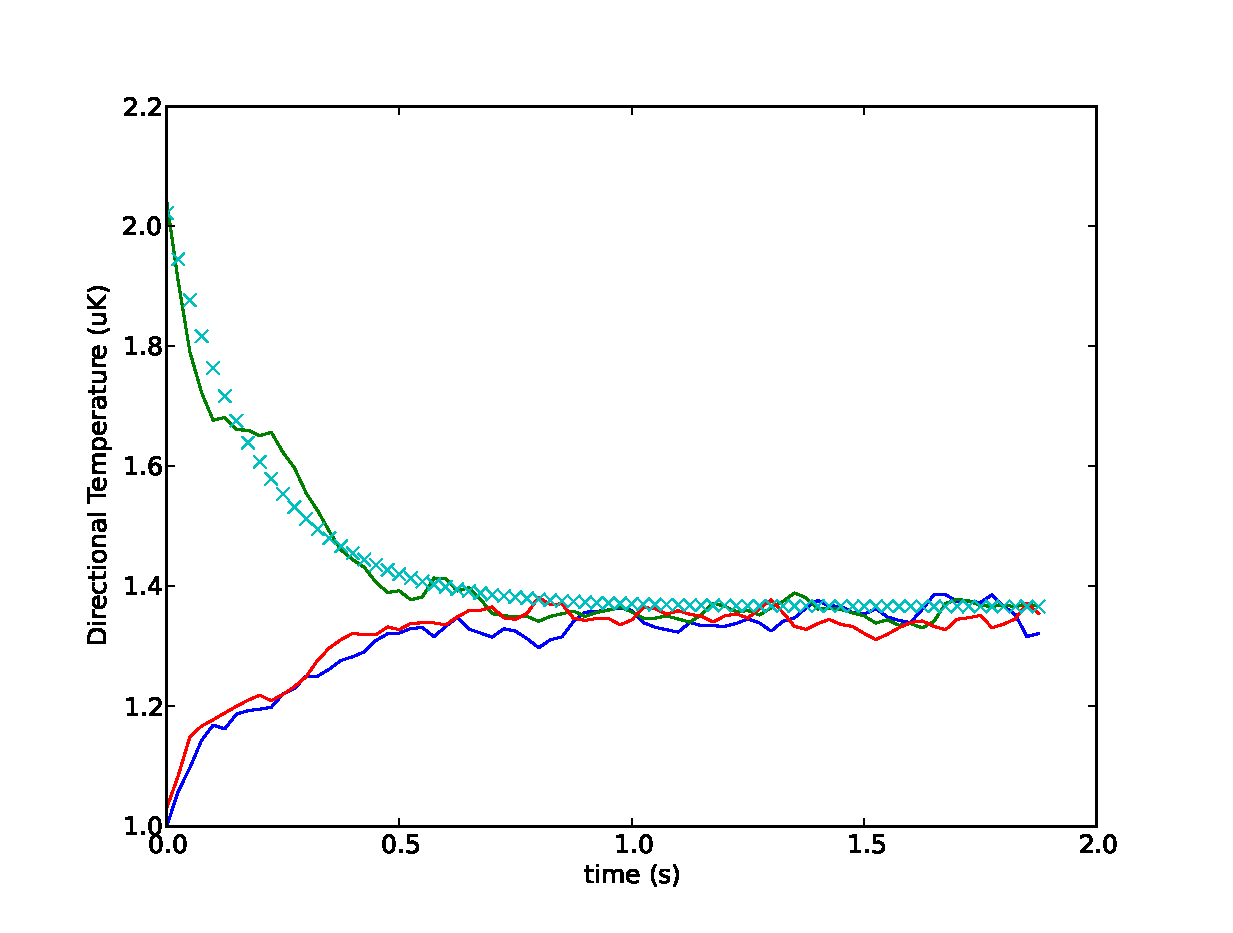
\includegraphics[width=.45\linewidth]{gfx/Thermalisation/monroeIP}}
\subfloat[Walraven quad gas thermalisation. $\tau_{c}^{-1} / \tau^{-1} = 6.09$]
{\label{fig:dsmcquaderr}
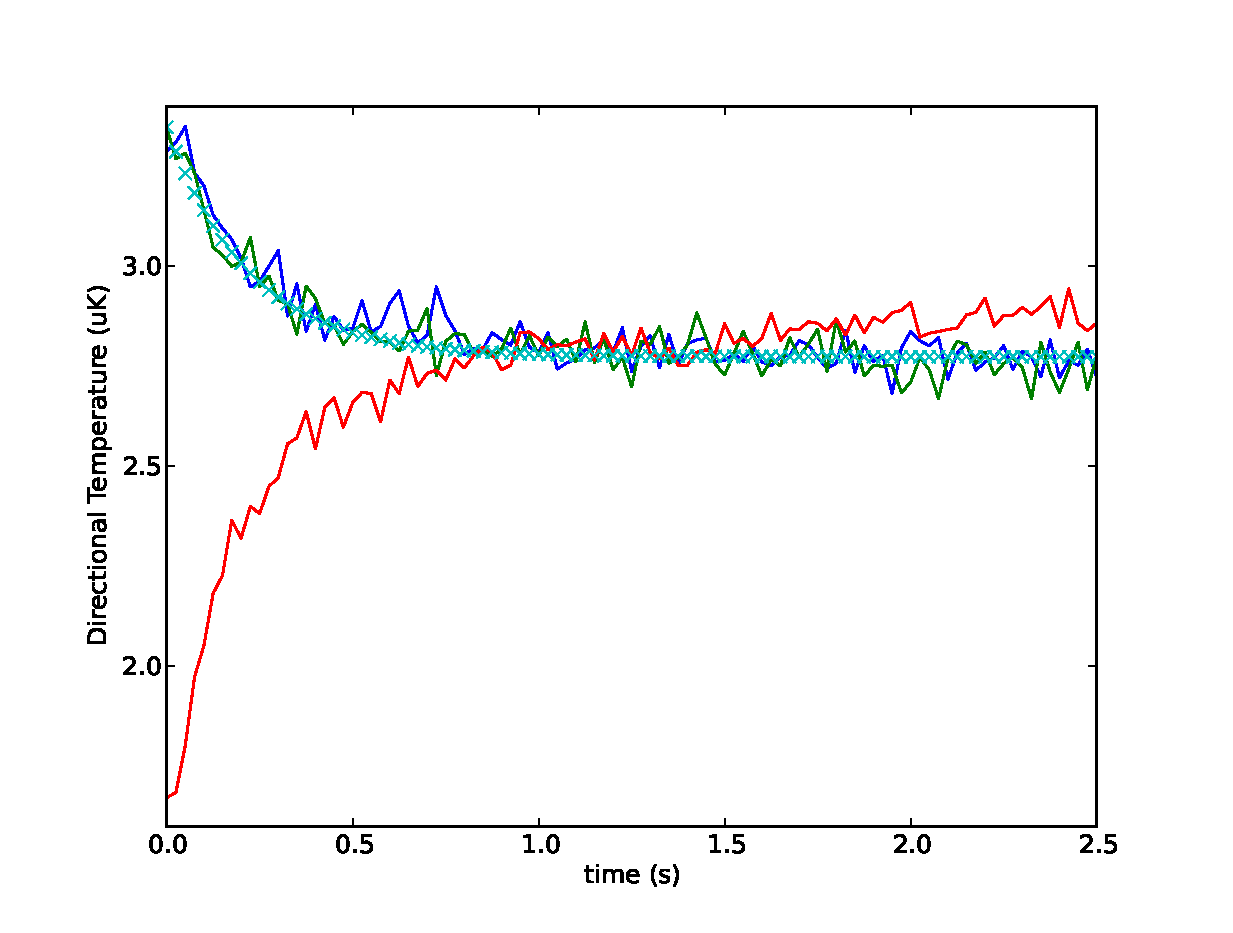
\includegraphics[width=.45\linewidth]{gfx/Thermalisation/monroeQuad}}
\caption[]{Error of DSMC method as a function of test particle number and cell number.}\label{fig:dsmccolerr}
\end{figure}

Also do it for different temperatures or trap numbers.

*** MUST REDO ALL OF THESE SIMULATIONS WITH COLLISIONS WORKING CORRECTLY (I.E. WITH THE NEW SORTING FIX IMPLEMENTED). ***

%----------------------------------------------------------------------------------------

\section{Evaporation}

Compare some results to those predicted by the theory of walraven and the other guy. 

\begin{figure}[bth]
\myfloatalign
\subfloat[$\eta$ should equal 7, here it is equal to 7.86 ]
{\label{fig:dsmchomoerr}
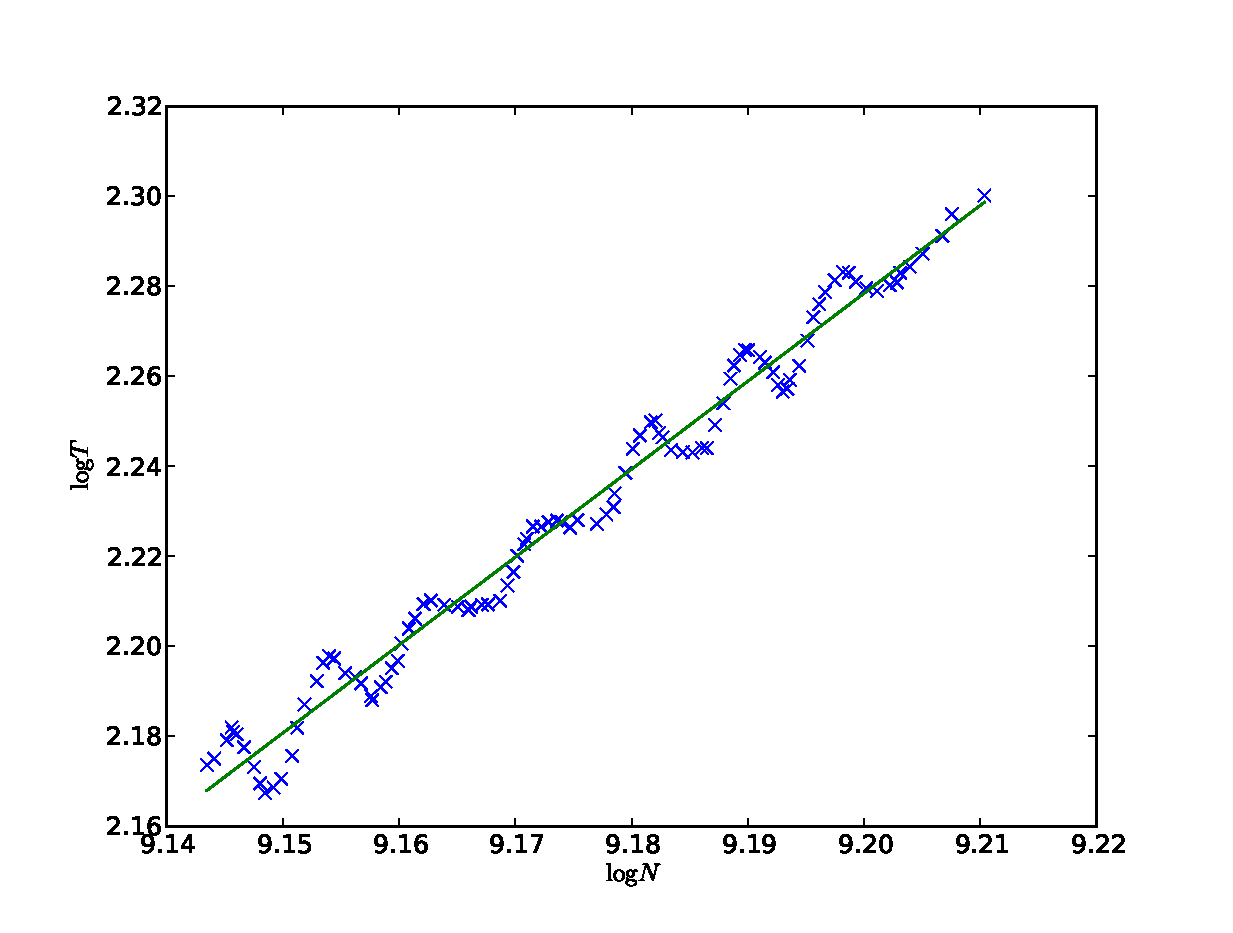
\includegraphics[width=.45\linewidth]{gfx/Evaporation/evapIP}} \quad
\subfloat[I want this to be a plot of n0 vs N.]
{\label{fig:dsmcquaderr}
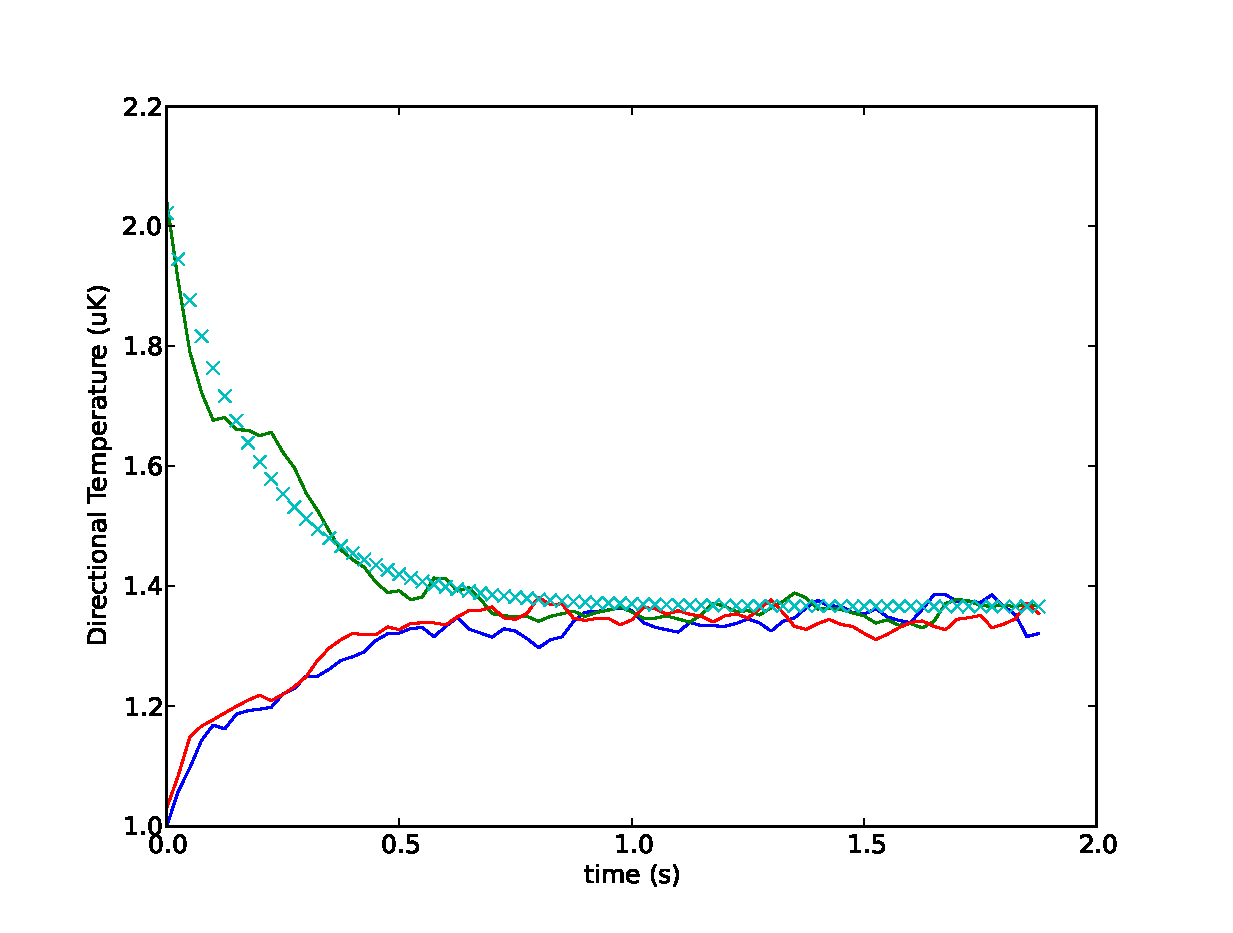
\includegraphics[width=.45\linewidth]{gfx/Thermalisation/monroeIP}}
\subfloat[Not sure what plot tp put here]
{\label{fig:dsmcquaderr}
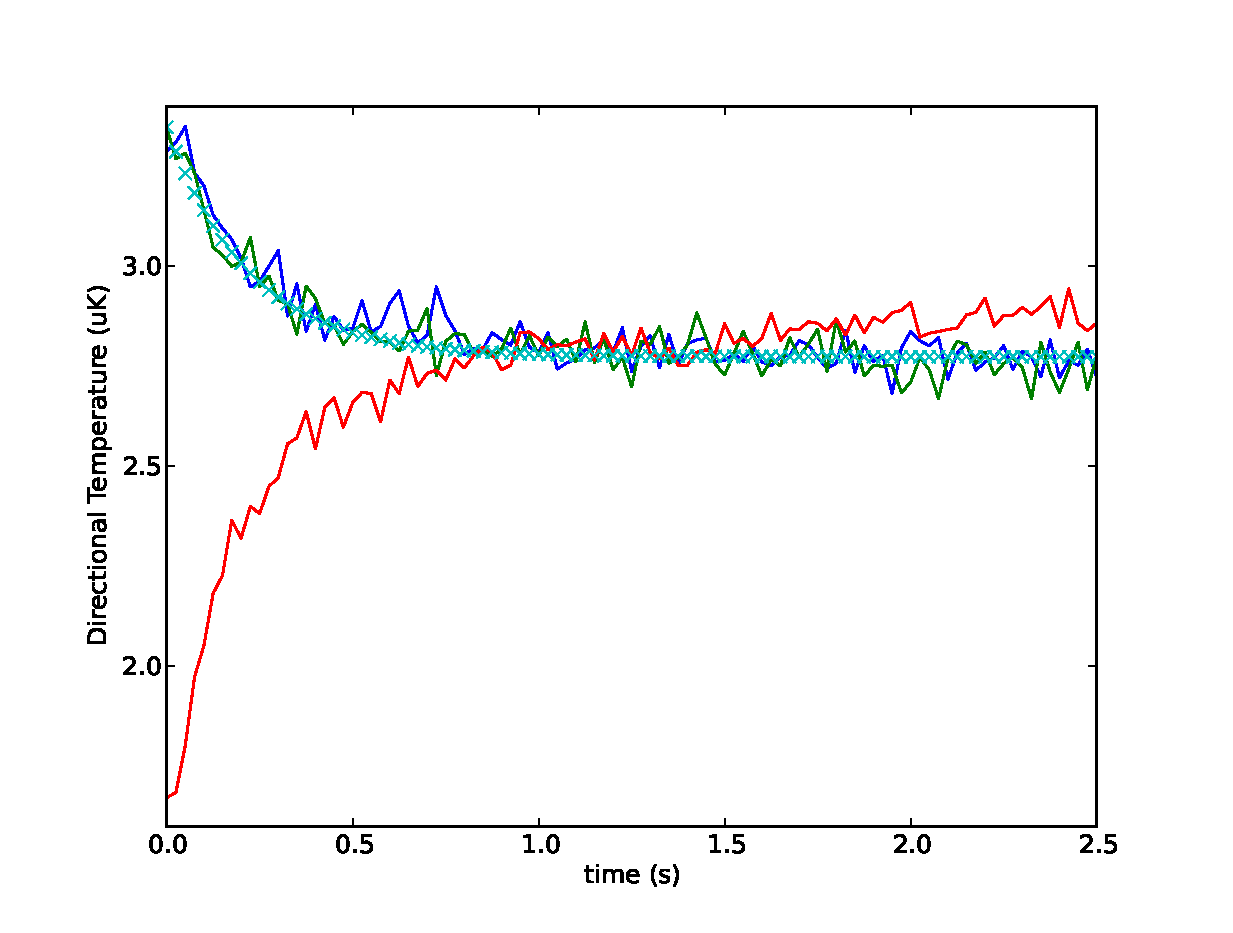
\includegraphics[width=.45\linewidth]{gfx/Thermalisation/monroeQuad}}
\caption[]{IP trap evaporation.}\label{fig:dsmccolerr}
\end{figure}

\begin{figure}[bth]
\myfloatalign
\subfloat[$\eta$ should equal ?(check the paper), here it is equal to 5 ]
{\label{fig:dsmchomoerr}
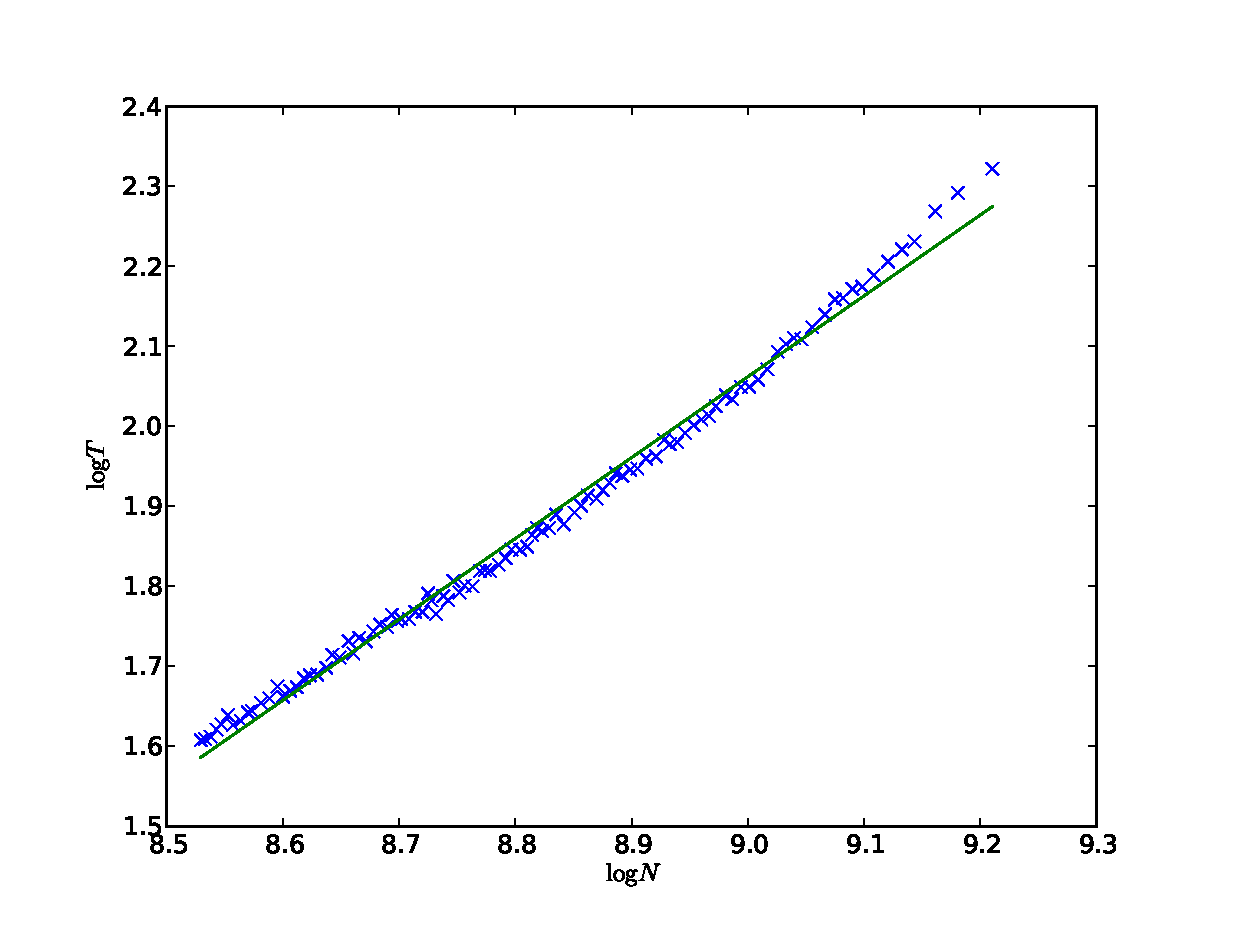
\includegraphics[width=.45\linewidth]{gfx/Evaporation/evapQuad}} \quad
\subfloat[I want this to be a plot of n0 vs N.]
{\label{fig:dsmcquaderr}
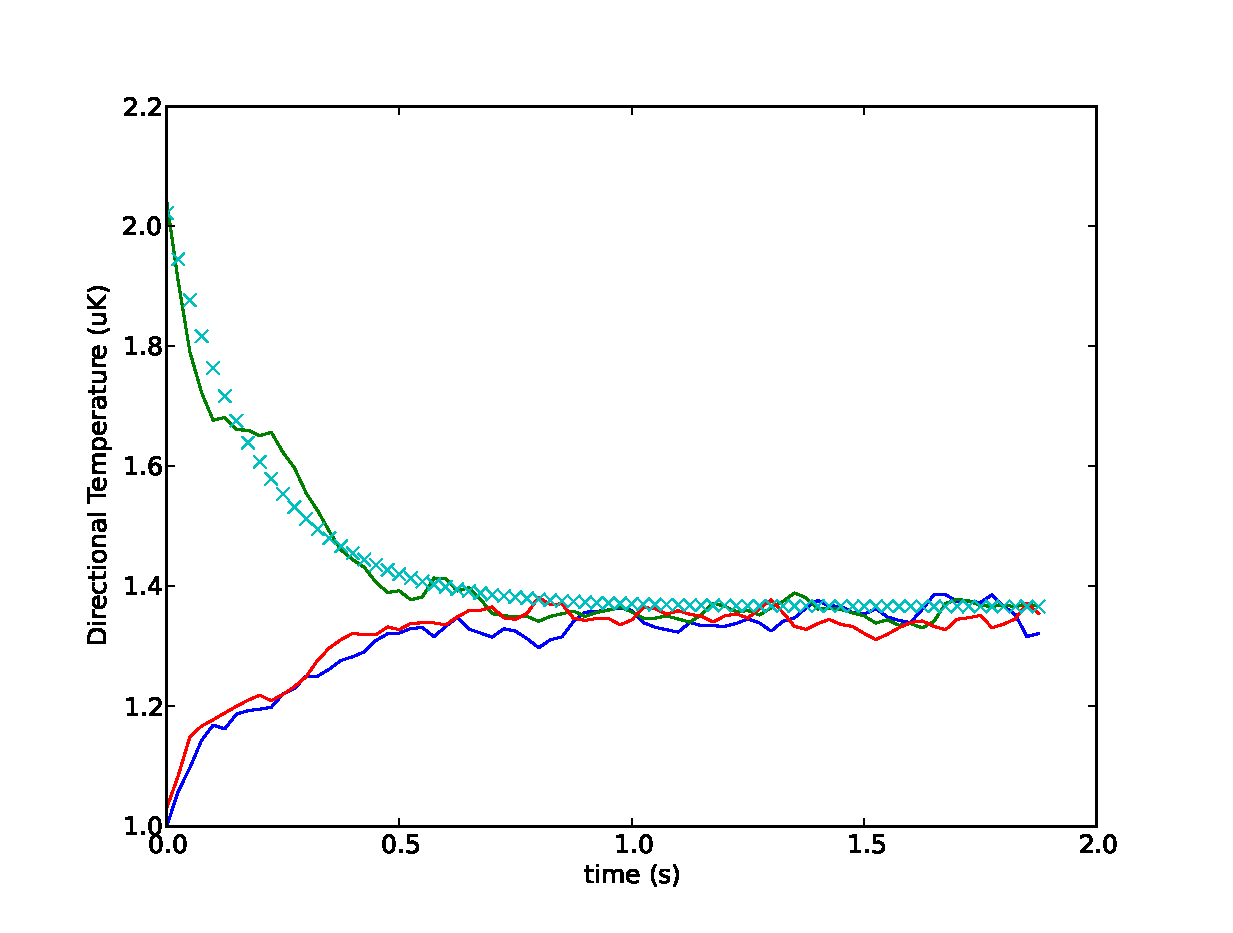
\includegraphics[width=.45\linewidth]{gfx/Thermalisation/monroeIP}}
\subfloat[Not sure what plot tp put here]
{\label{fig:dsmcquaderr}
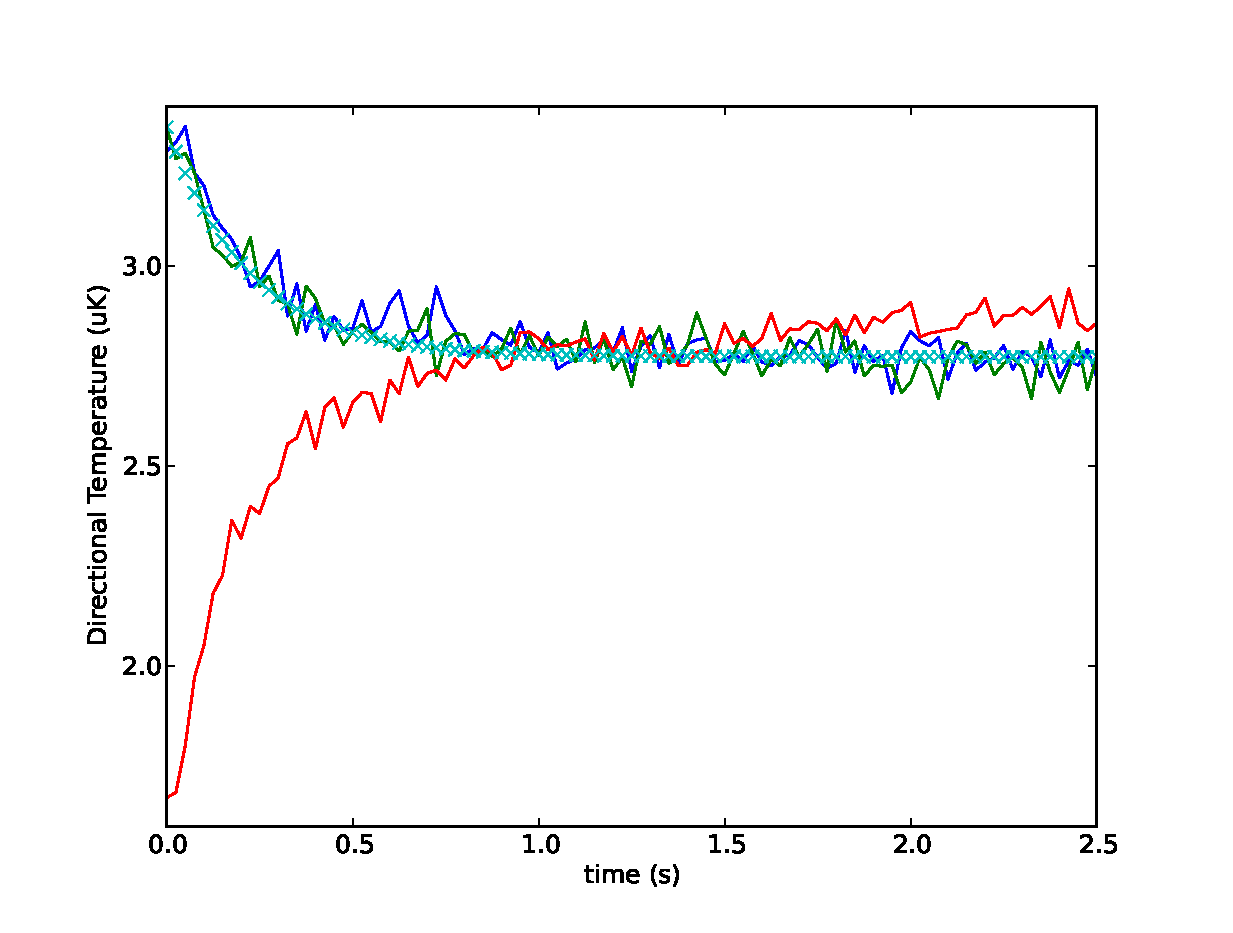
\includegraphics[width=.45\linewidth]{gfx/Thermalisation/monroeQuad}}
\caption[]{Quadrupole trap evaporation.}\label{fig:dsmccolerr}
\end{figure}

\section{Adiabaticity}

Have a look at squeezing the magnetic trap both diabaticaly and adiabatically.